\documentclass[final,t]{beamer}

% poster template
\usepackage[orientation=portrait,size=a0,scale=1.4,debug]{beamerposter}
\usetheme{zurichposter}
\usepackage{graphicx}
\usepackage{varwidth}
\usepackage{multirow}
% references
%\usepackage[bibstyle=authoryear, citestyle=authoryear-comp,%
%hyperref=auto]{biblatex}
%\bibliography{references}

\newcommand*\circled[1]{\tikz[baseline=(char.base)]{
            \node[shape=circle,draw,inner sep=2pt] (char) {#1};}}
%title

% document properties
\title{\LARGE HAShCache: Heterogeneity Aware Shared DRAMCache For Integrated Heterogenous Architectures}
\author{Adarsh Patil, R Govindarajan}
\institute{Department of CSA, Indian Institute of Science, Bangalore }


%------------------------------------------------------------------------------
\begin{document}

% my figures
\usetikzlibrary{shapes,arrows}
\usetikzlibrary{backgrounds}
\usetikzlibrary{matrix, positioning, fit}
\usetikzlibrary{patterns}
\definecolor{forestgreen}{rgb}{0.0, 0.5, 0.0}

\tikzstyle{smallcircle} =[fill=black!100, text=white, circle, inner sep=1pt, minimum size=0.1em]
\tikzstyle{ourcircle} = [draw, semicircle, inner sep=0pt,minimum size=2pt]
\tikzstyle{dullblock} = [draw, fill=black!20, circle, minimum height=2em, minimum width=2em]
\tikzstyle{block} = [draw=black, rounded corners, thick, line width=0.3mm, rectangle, minimum height=10em, minimum width=7em]
\tikzstyle{blocksmall} = [draw=black, thick, line width=0.5mm, rectangle, minimum height=6em, minimum width=3em, fill=white]
\tikzstyle{group} = [draw=black, line width=0.3mm, rectangle, minimum height=2em, minimum width=2em]
\tikzstyle{textblock} = [draw, fill=black!20, rectangle, rounded corners]
\tikzstyle{rectblock} = [draw, rectangle, minimum height=1.3em]
\tikzstyle{plain} = []
\tikzstyle{decisionblock} = [draw, diamond, fill=black!20]
\tikzstyle{input} = [draw, thick, fill=blue!20, circle, minimum size=1pt]
\tikzstyle{output} = [draw, fill=blue!20, circle, minimum size=1pt]
\tikzstyle{pinstyle} = [pin edge={to-,thin,black}]
\tikzset{toprule/.style={%
        execute at end cell={%
            \draw [line cap=rect,#1] (\tikzmatrixname-\the\pgfmatrixcurrentrow-\the\pgfmatrixcurrentcolumn.north west) -- (\tikzmatrixname-\the\pgfmatrixcurrentrow-\the\pgfmatrixcurrentcolumn.north east);%
        }
    },
    bottomrule/.style={%
        execute at end cell={%
            \draw [line cap=rect,#1] (\tikzmatrixname-\the\pgfmatrixcurrentrow-\the\pgfmatrixcurrentcolumn.south west) -- (\tikzmatrixname-\the\pgfmatrixcurrentrow-\the\pgfmatrixcurrentcolumn.south east);%
        }
    }
}


\newcommand{\bloom}[0]{
    \begin{tikzpicture}[auto, >=latex']
        % Blocks
        \node [textblock, thick, minimum height=5em] (bye){\begin{varwidth}{4cm} \centering{\footnotesize{B\\y\\E\\}} \end{varwidth}};
        \node [textblock, thick, minimum width=6em, minimum height=4em, right = 1.5cm of bye, yshift=2.2cm] (dramcache){\begin{varwidth}{4cm} \centering{\footnotesize{DRAM\\Cache}} \end{varwidth}};
        \node [textblock, thick, left = 0.01cm of dramcache, xshift=1.5em] (pred){\begin{varwidth}{4cm} \centering{\tiny{P\\R\\E\\D\\}} \end{varwidth}};
        \node [textblock, thick, left = 0.01cm of dramcache] (queue){\begin{varwidth}{4cm} \centering{\footnotesize{I I I I}} \end{varwidth}};
        \node [textblock, thick, minimum width=4em, right = 5cm of bye, minimum height=7em, yshift=-0.5cm] (dram){\begin{varwidth}{4cm} \centering{\footnotesize{Off-Chip\\DRAM\\Memory}} \end{varwidth}};

        % Arrows
        \draw [<-,very thick] (bye.west) to [out=180,in=0] ++(-0.6,0);
        \draw [->, very thick] (dramcache.east) to [out=0,in=180] ++(2.1,0) to (dram.north);
        \draw [->, very thick] ([yshift=1em]dramcache.east) to [out=0,in=180] ++(3.5,0);
        \draw [->, very thick] (dram.east) to [out=0,in=180] ++(1.1,0);
        \draw [<-, very thick] (queue.south) to ++(0.12,-0.85) to [out=180,in=0] ++(-1.35,0) to (bye.north);
        \draw [->, very thick] (dramcache.south) to [out=-90,in=90] ++(0,-0.8) to [out=180,in=0] ++(-2.6,0);
        \draw [->, very thick] ([yshift=2.5em] dram.west) to ++(-1.6,0) to ([xshift=2.3em] dramcache.south);
        \draw [<->, very thick] (bye.south) to [out=-90,in=90] ++(0,-0.5) to [out=0,in=180] ++(5.25,0);
        \draw [->, very thick] (bye.east) to [out=0,in=180] ++(5,0);
        \draw [<-, very thick] (queue.west) to ++(-0.45,0.45) to ++(-1,0);
        \draw [<-, very thick] (queue.west) to ++(-0.45,-0.45) to ++(-1,0);
        \draw [-, very thick, xshift=3.2cm] (0,1.5) to (0,0.16);
        \draw [-, very thick, xshift=3.2cm, right=90, looseness=3] (-0.07,0.067) to (0,-0.15);
        \draw [->, very thick, xshift=3.2cm] (0.01,-0.13) to (0,-1.4);
        \draw [->, dashed] (pred.east) to [out=0,in=180] ++(1.65,0);

        % labels
        \node [plain, left=0.01cm of bye, minimum height=1em, minimum width=1em] (cpurd) {\begin{varwidth}{4cm}\scriptsize{CPU\\ \\Rd}\end{varwidth}};
        \node [plain, above=1.4cm of dram, minimum height=1em, minimum width=1em, xshift=-2.8em, yshift=-1.8em] (cachemiss) {\begin{varwidth}{4cm}\scriptsize{Cache Miss/\\Pred Off-chip acess}\end{varwidth}};
        \node [plain, left=1.2cm of dram, minimum height=1em, minimum width=1em, yshift=-3em] (dirtyevict) {\begin{varwidth}{4cm}\scriptsize{Dirty Eviction}\end{varwidth}};
        \node [plain, left=0.4cm of dramcache, minimum height=1em, minimum width=1em, yshift=-1.44em, xshift=-2em] (WrReq) {\begin{varwidth}{4cm}\scriptsize{CPU Wr\\ Req}\end{varwidth}};
        \node [plain, left=0.3cm of dramcache, minimum height=1em, minimum width=1em, yshift=1.2em, xshift=-1.8em] (GpuReq) {\begin{varwidth}{4cm}\scriptsize{GPU Rd/Wr \\Req}\end{varwidth}};
        \node [plain, right=0.2cm of bye, minimum height=1em, minimum width=1em, yshift=1.25cm, xshift=-0.5cm] (maydir) {\begin{varwidth}{4cm}\scriptsize{Maybe Dirty}\end{varwidth}};
        \node [plain, right=0.2cm of bye, minimum height=1em, minimum width=1em, yshift=0.1cm, xshift=1cm] (notdir) {\begin{varwidth}{4cm}\scriptsize{Not Dirty}\end{varwidth}};
        \node [plain, below=0.15cm of maydir, minimum height=1em, minimum width=1em, xshift=1cm, yshift=0.2cm] (wrhit) {\begin{varwidth}{4cm}\scriptsize{Write Hit}\end{varwidth}};
        \node [plain, left=0.01cm of dram, minimum height=1em, minimum width=1em, yshift=3em] (fill) {\begin{varwidth}{4cm}\scriptsize{GPU Fill}\end{varwidth}};
        \node [plain, above=0.01pt of queue, minimum height=1em, minimum width=1em, yshift=-0.3em] (reqq) {\begin{varwidth}{4cm}\scriptsize{Req Q}\end{varwidth}};
        \node [plain, right=0.01pt of dram, minimum height=1em, minimum width=1em] (cpubypass) {\begin{varwidth}{4cm}\scriptsize{CPU Resp\\Bypass}\end{varwidth}};
        \node [plain, right=1.5cm of dramcache, minimum height=1em, minimum width=1em, yshift=1em] (datadram) {\begin{varwidth}{4cm}\scriptsize{Resp from\\ DRAM Cache}\end{varwidth}};


    \end{tikzpicture}

}

\newcommand{\chainaccess}[0]{
    \begin{tikzpicture}[auto, >=latex']
        % We start by placing the blocks
        \node [textblock, thick, minimum width=6em] (act){\begin{varwidth}{4cm} \centering{\footnotesize{DRAM $\$$ \\Row Act.}} \end{varwidth}};
        \node [textblock, thick, right = 0.5cm of act, minimum width=4em] (burst) {\begin{varwidth}{4cm} \centering{\footnotesize{TAD \\Burst}} \end{varwidth}};
        \node [decisionblock, thick, right = 0.5cm of burst] (tagmatch) {\begin{varwidth}{4cm} \centering{\scriptsize{Tag\\Match}} \end{varwidth}};
        \node [textblock, thick, below = 0.5cm of tagmatch] (chaintable) {\begin{varwidth}{4cm} \centering{\footnotesize{Chain\\Offset}} \end{varwidth}};
        \node [decisionblock, thick, right = 1.8cm of tagmatch.south] (clean) {\begin{varwidth}{4cm} \centering{\scriptsize{Clean?}} \end{varwidth}};
        \node [decisionblock, thick, right = 2.1cm of tagmatch, yshift=1.5em] (pamreturn) {\begin{varwidth}{4cm} \centering{\scriptsize{PAM \\return?}} \end{varwidth}};
        \node [textblock, thick, right = 1.5cm of pamreturn.south, minimum width=4em, yshift=-1em] (chaintad) {\begin{varwidth}{4cm} \centering{\footnotesize{Chain\\TAD}} \end{varwidth}};
        \node [decisionblock, thick, right = 0.5cm of chaintad] (chainmatch) {\begin{varwidth}{4cm} \centering{\scriptsize{Tag\\Match}} \end{varwidth}};
        \node [textblock, thick, right = 0.5cm of chainmatch, minimum height=7em, yshift=1.5em] (mem) {\begin{varwidth}{4cm} \centering{\footnotesize{Off-chip\\DRAM\\Memory}} \end{varwidth}};

        % Arrows
        \draw [->,very thick] (act) -- (burst);
        \draw [->,very thick, red] (chaintable.east) -- (clean);
        \draw [->,very thick] (burst) -- (tagmatch);
        \draw [->,very thick] (tagmatch.south) -- (chaintable.north);
        \draw [->,very thick] (tagmatch.east) to [out=0,in=180] ++(0.5,0) to [out=90,in=-90] ++(0,1.5);
        \draw [->,very thick, red] (clean.north) to [out=90,in=-90] ++(0,0.65) to (pamreturn.west);
        \draw [->,very thick, red] (pamreturn.south)to [out=-90,in=90] ++(0,-0.3) to [out=0,in=180] ++(1.5,0);
        \draw [->,very thick, red] (pamreturn.east) to [out=0,in=180] ++(0.5,0) to [out=90,in=-90] ++(0,0.5);
        \draw [->,very thick, red] (clean.east) to [out=0,in=180] ++(2.2,0);
%        \draw [->,very thick] (chaintable.south) to [out=0,in=180] ++(9.65,0) to (mem.south);
        \draw [->,very thick] (chainmatch.east) to [out=0,in=180] ++(0.6,0);
        \draw [->,very thick] (chaintad.east) -- (chainmatch);
        \draw [->,very thick] (chainmatch.north) to [out=90,in=-90] ++(0,1);
        \draw [->,very thick] (chaintable.east) to [out=0,in=180] ++(5.7,0) to (chaintad.south);
        \draw [->,very thick] (chaintable.east) to [out=0,in=180] ++(0.3,-0.4) to [out=0,in=180] ++(9.65,0) to (mem.south);

        % Groups
        \node [blocksmall, draw=white, above = 1cm of clean, minimum height=1em, minimum width=0.2em, xshift=-0.7em, yshift=0.4em] (lblcpu){\textbf{CPU}};
        \node[group, dashed, inner sep = 1pt, line width=0.3mm, draw=red, fit=(clean)(pamreturn)] (cpugroup) {};

        % Labels
        \node [plain, right=0.01em of tagmatch, minimum height=1em, minimum width=1em, yshift=1em, xshift=-0.5em] (lbl1) {\footnotesize{\emph{Hit}}};
        \node [plain, below=0.01em of tagmatch, minimum height=1em, minimum width=1em, xshift=-1.2em] (lbl2) {\footnotesize{\emph{Miss}}};
        \node [plain, below=0.52cm of tagmatch, minimum height=1em, minimum width=1em, xshift=4em] (lbl3) {\footnotesize{\emph{Yes}}};
        \node [plain, below=0.1cm of lbl3, minimum height=1em, minimum width=1em, yshift=0.2em] (lbl4) {\footnotesize{\emph{No}}};
        \node [plain, above=0.01cm of lbl3, minimum height=1em, minimum width=1em, red] (lb15) {\footnotesize{\emph{Yes}}};
        \node [plain, right=0.01em of chainmatch, minimum height=1em, minimum width=1em, yshift=-0.5em, xshift=-0.65em] (lbl5) {\footnotesize{\emph{Miss}}};
        \node [plain, above=3em of lbl5, minimum height=1em, minimum width=1em, yshift=-0.5em, xshift=-2em] (lbl8) {\footnotesize{\emph{Hit}}};
        \node [plain, right=0.01em of clean, minimum height=1em, minimum width=1em, yshift=-0.5em, red] (lbl6) {\footnotesize{\emph{No}}};
        \node [plain, right=2.5em of lbl6, minimum height=1em, minimum width=1em, yshift=1.5em, xshift=-1.5em, red] (lbl7) {\footnotesize{\emph{No}}};
        \node [plain, above=1.8em of clean, minimum height=1em, minimum width=1em, xshift=-0.1em, red] (lbl9) {\footnotesize{\emph{Yes}}};
        \node [plain, above=1.8em of chaintad, minimum height=1em, minimum width=1em, yshift=0.5em, xshift=-1.5em, red] (lbl10) {\footnotesize{\emph{Yes}}};
        \node [plain, above=0.3em of lbl10, minimum height=1em, minimum width=1em] (lbl11) {\footnotesize{\emph{Return Data}}};
        \node [plain, left=9.7em of lbl11, minimum height=1em, minimum width=1em] (lbl12) {\footnotesize{\emph{Return Data}}};
        \node [plain,right =2.5em of lbl11, minimum height=1em, minimum width=1em] (lbl13) {\footnotesize{\emph{Return Data}}};

        % Row Buffer
        \node [rectblock, thick, above = 2.4cm of act, minimum width=6.5em] (data) {\begin{varwidth}{4cm} \centering{\footnotesize{DATA}} \end{varwidth}};
        \node [rectblock, thick, right = 0cm of data, minimum width=4em] (tag) {\begin{varwidth}{4cm} \centering{\footnotesize{TAG}} \end{varwidth}};
        \node [rectblock, thick, right = 0cm of tag, minimum width=1pt] (isgpu) {\begin{varwidth}{4cm} \centering{\scriptsize{}} \end{varwidth}};
        \node [rectblock, thick, right = 0cm of isgpu] (chain) {\begin{varwidth}{4cm} \centering{\scriptsize{}} \end{varwidth}};
        \node [rectblock, thick, right = 0cm of chain] (reversechain) {\begin{varwidth}{4cm} \centering{\scriptsize{}} \end{varwidth}};
        \node [rectblock, thick, right = 0cm of reversechain, minimum width=1pt] (chaindirty) {\begin{varwidth}{4cm} \centering{\scriptsize{}} \end{varwidth}};
        \node [rectblock, thick, right = 0cm of chaindirty, minimum width=9em] (tad2) {\begin{varwidth}{4cm} \centering{\scriptsize{\textbf{TAD 2}}} \end{varwidth}};
        \node [rectblock, thick, right = 0cm of tad2, minimum width=8em] (row) {\begin{varwidth}{4cm} \centering{\textbf{...}} \end{varwidth}};
        \node [rectblock, thick, right = 0cm of row, minimum width=9em] (tad15) {\begin{varwidth}{4cm} \centering{\scriptsize{\textbf{TAD 15}}} \end{varwidth}};
        \node [rectblock, thick, right = 0cm of tad15, minimum width=1.2em] (cg) {\begin{varwidth}{4cm} \centering{} \end{varwidth}};
        \node [rectblock, thick, right = 0cm of cg, minimum width=2em, pattern=north west lines] (dc) {\begin{varwidth}{4cm} \centering{} \end{varwidth}};
        \draw [decorate,decoration={brace,amplitude=5pt},yshift=8.7em, xshift=-2.8em] (0,0.3) -- (4.6,0.3) node [black,midway,yshift=0.5em] {\footnotesize \textbf{TAD 1} ($128B + 8B$)};
        \draw [decorate,decoration={brace,amplitude=5pt},yshift=8.7em, xshift=3.2em] (11.75,0.3) -- (12.9,0.3) node [black,midway,yshift=0.5em] {\footnotesize $8B$ unused};

        \node [plain, below=0.4cm of chain, minimum height=1em, minimum width=1em, xshift=-1.6em] (lbl31){\begin{varwidth}{4cm} \centering{\footnotesize{2bit Chain}} \end{varwidth}};
        \node [plain, below=0.7cm of reversechain, minimum height=1em, minimum width=1em, xshift=1em] (lbl32) {\begin{varwidth}{4cm} \centering{\footnotesize{2bit Reverse Chain}} \end{varwidth}};
        \node [plain, below=0.2cm of chaindirty, minimum height=1em, minimum width=1em, xshift=2.4em] (lbl33) {\begin{varwidth}{4cm} \centering{\footnotesize{1bit Chain Dirty}} \end{varwidth}};
        \node [plain, below=0.1cm of cg, minimum height=1em, minimum width=1em, xshift=1em] (lbl34) {\begin{varwidth}{4cm} \centering{\footnotesize{CPU/GPU bitvector(15 bits)}} \end{varwidth}};
        \node [plain, below=0.1cm of isgpu, minimum height=1em, minimum width=1em, xshift=-1.8em] (lbl35) {\begin{varwidth}{4cm} \centering{\footnotesize{CPU/GPU}} \end{varwidth}};

        \draw [<-] (chain.south) to [out=-90,in=90] ++(0,-0.5);
        \draw [<-] (reversechain.south) to [out=-90,in=90] ++(0,-0.8);
        \draw [<-] (chaindirty.south) to [out=-90,in=90] ++(0,-0.3);
        \draw [<-] (cg.south) to [out=-90,in=90] ++(0,-0.2);
        \draw [<-] (isgpu.south) to [out=-90,in=90] ++(0,-0.2);

    \end{tikzpicture}
}

\newcommand{\hsacpu}[0]{
    \begin{tikzpicture}[auto, >=latex']
        %CPU
        \node [blocksmall, minimum height=1em, minimum width=1em] (cpu1) {\begin{varwidth}{4cm}\centering{CPU\\ Core 1} \end{varwidth}};
        \node [blocksmall, above = 0.1cm of cpu1, minimum height=1em, minimum width=1em] (l11){\begin{varwidth}{4cm} \centering{L1} \end{varwidth}};
        
        %\node [blocksmall, right = 0.1cm of cpu1, minimum height=1em, minimum width=1em] (cpu2) {\begin{varwidth}{4cm} \centering{CPU\\ Core 2} \end{varwidth}};
        %\node [blocksmall, above = 0.1cm of cpu2, minimum height=1em, minimum width=1em] (l12){\begin{varwidth}{4cm} \centering{L1} \end{varwidth}};
        
        \node [smallcircle, right=0.15cm of cpu1] (dot1) {};
        \node [smallcircle, right=0.05cm of dot1] (dot2) {};
        \node [smallcircle, right=0.05cm of dot2] (dot3) {};
        
        %\node [blocksmall, right = 0.1cm of cpu2, minimum height=1em] (cpu3){\begin{varwidth}{4cm} \centering{CPU\\ Core 3} \end{varwidth}};
        %\node [blocksmall, above = 0.1cm of cpu3, minimum height=1em] (l13){\begin{varwidth}{4cm} \centering{L1} \end{varwidth}};
        
        \node [blocksmall, right = 0.15cm of dot3, minimum height=1em, minimum width=1em] (cpu4){\begin{varwidth}{4cm} \centering{CPU\\ Core N} \end{varwidth}};
        \node [blocksmall, above = 0.1cm of cpu4, minimum height=1em, minimum width=1em] (l14){\begin{varwidth}{4cm} \centering{L1} \end{varwidth}};
        \node [blocksmall, above = 2.01cm of dot3, minimum height=3em, minimum width=6em] (l24){\begin{varwidth}{4cm} \centering{L2} \end{varwidth}};
        
       % \begin{scope}[on background layer]
            %\node[group, inner sep = 3pt, line width=0.3mm, draw=red, yshift=1em, fit=(cpu1)(cpu2)(cpu3)(cpu4)(l11)(l12)(l13)(l14)(l24)] (grpcpu) {};
       % \end{scope}
        
        
        %GPU
        \node [blocksmall, right = 0.6cm of cpu4, minimum height=1.5em, minimum width=1em] (sm1) {CU};
        \node [blocksmall, above = 0.1cm of sm1, minimum height=1pt, minimum width=1em] (sm1l1) {\scriptsize{L1}};
        \node [blocksmall, right = 0.15cm of sm1, minimum height=1.5em, minimum width=1em] (sm2) {CU};
        \node [blocksmall, above = 0.1cm of sm2, minimum height=1em, minimum width=1em] (sm2l1) {\scriptsize{L1}};
        \node [blocksmall, right = 0.15cm of sm2, minimum height=1.5em, minimum width=1em] (sm3) {CU};
        \node [blocksmall, above = 0.1cm of sm3, minimum height=1em, minimum width=1em] (sm3l1) {\scriptsize{L1}};
        \node [blocksmall, right = 0.15cm of sm3, minimum height=1.5em, minimum width=1em] (sm4) {CU};
        \node [blocksmall, above = 0.1cm of sm4, minimum height=1em, minimum width=1em] (sm4l1) {\scriptsize{L1}};
        \node [blocksmall, above = 2.3cm of sm1, minimum height=1.5em, minimum width=1em] (sm5) {CU};
        \node [blocksmall, below = 0.1cm of sm5, minimum height=1em, minimum width=1em] (sm5l1) {\scriptsize{L1}};
        \node [blocksmall, right = 0.15cm of sm5, minimum height=1.5em, minimum width=1em] (sm6) {CU};
        \node [blocksmall, below = 0.1cm of sm6, minimum height=1em, minimum width=1em] (sm6l1) {\scriptsize{L1}};
        \node [blocksmall, right = 0.15cm of sm6, minimum height=1.5em, minimum width=1em] (sm7) {CU};
        \node [blocksmall, below = 0.1cm of sm7, minimum height=1em, minimum width=1em] (sm7l1) {\scriptsize{L1}};
        \node [blocksmall, right = 0.15cm of sm7, minimum height=1.5em, minimum width=1em] (sm8) {CU};
        \node [blocksmall, below = 0.1cm of sm8, minimum height=1em, minimum width=1em] (sm8l1) {\scriptsize{L1}};  
        
        \node [blocksmall, minimum height=1.1em, minimum width=6em] at (5.6,1.45)
        (l2gpu) {\begin{varwidth}{4cm} \centering{\small{Coherent GPU \\L2}}\end{varwidth}};
        
         %\begin{scope}[on background layer]
            \node[group, inner sep = 3pt, line width=0.3mm, draw=red, fit=(sm1)(sm1l1)(sm2)(sm2l1)(sm3)(sm3l1)(sm4)(sm4l1)(sm5)(sm5l1)(sm6)(sm6l1)(sm7)(sm7l1)(sm8)(sm8l1)(l2gpu)] (grpgpu) {};
         %\end{scope}                        
        
        
        %Interconnect
        \node [blocksmall, minimum height=1.5em, minimum width=10.7em] at (1.5,1.5)
        (interconnect) {Cache Coherent Interconnect};
                
        %Connections to interconnect
        \draw [-,very thick] (l11.north) to ++(0, 0.15); 
        \draw [-, very thick] (l24.south) to ++(0, -0.3);
        \draw [-, very thick] (l2gpu.west) to ++(-0.82,0);
        \draw [-, very thick] (l14.north) to ++(0, 0.15);
        %\draw [-, very thick] (l13.north) to ++(0, 0.15);
        %\draw [-, very thick] (l12.north) to ++(0, 0.15);
        
        % Memory Controller
        \node [blocksmall, minimum height=1em, minimum width=9em, below=0.1cm of cpu4, xshift=-2em] (mc1){\begin{varwidth}{4cm} \centering{Memory Controller} \end{varwidth}};
        \node [blocksmall, minimum height=1em, minimum width=9em, right=0.05cm of mc1] (mc2){\begin{varwidth}{4cm} \centering{Memory Controller} \end{varwidth}};  
        
        %\draw [-, very thick] (-0.78,-0.6) to (-0.78, 1.5) to (interconnect.west);
        \draw [-, very thick] (2.8,-0.6) to (2.8, 1.25);
        \draw [-, very thick] (3.07,-0.6) to (3.07, 1.25);
        
        %Chip
        \begin{scope}[on background layer]
             \node[group, inner sep = 4pt, line width=0.6mm, fill=cyan!70, fit=(cpu1)(cpu4)(l11)(l14)(l24)(interconnect)(mc1)(mc2)(grpgpu)] (grpchip) {};
        \end{scope}

        % GPU L1 to L2 connections
        \draw [-,very thick] (sm1l1.north east) -- (l2gpu);
        \draw [-,very thick] (sm2l1.north) -- (l2gpu);
        \draw [-,very thick] (sm3l1.north) -- (l2gpu);
        \draw [-,very thick] (sm4l1.north) -- (l2gpu);
        \draw [-,very thick] (sm5l1.south east) -- (l2gpu);
        \draw [-,very thick] (sm6l1.south) -- (l2gpu);
        \draw [-,very thick] (sm7l1.south) -- (l2gpu);                
        \draw [-,very thick] (sm8l1.south) -- (l2gpu);

        % Off package Region
        \node [blocksmall, below = 3em of mc1, draw=black!30, fill=black!30, minimum height=0.5em, minimum width=7em] (mm1){};
%        \node [blocksmall, draw=blue, right = 0.2cm of mm1, minimum height=1.2em, minimum width=1.2em] (mm2){};
 %       \node [blocksmall, draw=blue, right = 0.2cm of mm2, minimum height=1.2em, minimum width=1.2em] (mm3){};
  %      \node [blocksmall, draw=blue, right = 0.2cm of mm3, minimum height=1.2em, minimum width=1.2em] (mm4){};
        
        \node [blocksmall, draw=black!30, fill=black!30, minimum height=0.5em, right = 0.8cm of mm1, minimum width=7em] (mm7){};
%        \node [blocksmall, draw=blue, right = 0.2cm of mm7, minimum height=1.2em, minimum width=1.2em] (mm8){};
%        \node [blocksmall, draw=blue, right = 0.2cm of mm8, minimum height=1.2em, minimum width=1.2em] (mm9){};
%        \node [blocksmall, draw=blue, right = 0.2cm of mm9, minimum height=1.2em, minimum width=1.2em] (mm10){};
        
        \node [blocksmall, draw=white, xshift=4em, below = 0.5cm of mm7, minimum height=1em, minimum width=1.2em] (lbl1){DIMMs};
        \node [blocksmall, draw=white, yshift=-4em, xshift=-13em, above = 0.1cm of mm7.south east, minimum height=1em, minimum width=1.2em] (lbl2){Off Package region};
        
        
        % Memory Grouping
        \begin{scope}[on background layer]
              \node[group, inner sep = 1pt, line width=0.6mm, fill=black!30, fit=(mm1)] (mmgrp1) {};
        \end{scope}
        \begin{scope}[on background layer]
              \node[group, inner sep = 1pt, line width=0.6mm, fill=black!30, fit=(mm7)] (mmgrp2) {};
        \end{scope}
        \node[group, inner sep = 3pt, line width=0.3mm, fit=(mmgrp1)(mmgrp2)(lbl1)(lbl2)] (mmgrp3) {};
        
        \draw [-,very thick, xshift=-2em] (1.2,-2.7) to (1.2, -3) to (3,-3) to (3,-2.7);
        \draw [-,very thick, xshift=7em,] (1.2,-2.7) to (1.2, -3) to (3,-3) to (3,-2.7);
%        \draw [-,very thick] (1.5,-2.15) to (1.5, -2.35) to (4.9,-2.35) to (4.9,-2.15);

        % Big Arrows
        \node[double arrow, draw, right = 0.1mm of grpchip.south, yshift=1em,
        rotate=-90, minimum height=3em, minimum width=1.3em, line width=0.5mm, fill=white](arrow2){};

    \end{tikzpicture}
}

\newcommand{\stackdram}[0]{
    \begin{tikzpicture}[auto, >=latex']
        %DRAM Cache  
        \node [block, draw=red, dashed, minimum height=7em, minimum width=4em] at (0,6.2) (sid){\begin{varwidth}{4cm} \centering{\footnotesize{Silicon\\ interposed\\ DRAM}} \end{varwidth}};
        
        \node [block, draw=red, right = 2.1cm of sid, dashed, minimum height=7em, minimum width=4em] (sid1){\begin{varwidth}{4cm} \centering{\footnotesize{Silicon\\ interposed\\ DRAM}} \end{varwidth}};
        
        \node [block, draw=red, minimum height=0.1pt, rounded corners=1pt, inner sep=1pt, minimum width=16em] at (1.77, 4.8) (blk1){\begin{varwidth}{4cm} \end{varwidth}};
        
        \node [block, draw=black, above = 0.05cm of blk1, minimum height=0.1em, minimum width=1em] (cpud){\begin{varwidth}{4cm} \centering{\scriptsize{CPU-GPU Die}} \end{varwidth}};
        
        \node [block, draw=red, above = 0.2cm of cpud, minimum height=4em, dashed, minimum width=4em] (vsd) {\begin{varwidth}{4cm} \centering{\footnotesize{Vertically\\ Stacked\\ DRAM\\}} \end{varwidth}};
        
        \node [blocksmall, draw=white, above = 0.01cm of sid.north east, minimum height=1em, minimum width=0.2em] (lbl3){\footnotesize{On Package region}};
        
        \node[group, inner sep=7pt, rounded corners, fit=(sid)(vsd)(sid1)(cpud)(blk1)(lbl3)] (g1) {};
        
        % TSV        
        \draw [-,very thick] (1.35,5.38) to (1.35,5.6);
        \draw [-,very thick] (1.65,5.38) to (1.65,5.6);
        \draw [-,very thick] (1.95,5.38) to (1.95,5.6);
        \draw [-,very thick] (2.25,5.38) to (2.25,5.6);
        
        % semicircles
        \node [smallcircle] at (-0.6,4.9) (s4) {};
        \node [smallcircle] at (-0.3,4.9) (s1) {};
        \node [smallcircle] at (0,4.9) (s2) {};
        \node [smallcircle] at (0.3,4.9) (s3) {};
        \node [smallcircle] at (0.6,4.9) (s4) {};
        %\node [smallcircle] at (0.7,4.9) (s3) {};
        %\node [smallcircle] at (1.0,4.9) (s4) {};

        \node [smallcircle] at (1,4.9) (s5) {};
        \node [smallcircle] at (1.3,4.9) (s6) {};
        \node [smallcircle] at (1.6,4.9) (s7) {};
        \node [smallcircle] at (1.9,4.9) (s8) {};
        \node [smallcircle] at (2.2,4.9) (s9) {};
        \node [smallcircle] at (2.5,4.9) (s10) {};

        \node [smallcircle] at (3.1,4.9) (s11) {};
        \node [smallcircle] at (3.4,4.9) (s12) {};
        \node [smallcircle] at (3.7,4.9) (s13) {};
        \node [smallcircle] at (4,4.9) (s14) {};
        \node [smallcircle] at (4.3,4.9) (s15) {};
        
\iffalse        
        % Off package Region
        \node [blocksmall, draw=black!30, fill=black!30, minimum height=0.5em, minimum width=0.5em] at (5.65,5.15)(mm1){};
        \node [blocksmall, draw=black!30, fill=black!30, above = 0.15cm of mm1, minimum height=0.5em, minimum width=0.5em] (mm2){};
        \node [blocksmall, draw=black!30, fill=black!30, above = 0.15cm of mm2, minimum height=0.5em, minimum width=0.5em] (mm3){};
        \node [blocksmall, draw=black!30, fill=black!30, above = 0.15cm of mm3, minimum height=0.5em, minimum width=0.5em] (mm4){};
        \node [blocksmall, draw=black!30, fill=black!30, above = 0.15cm of mm4, minimum height=0.5em, minimum width=0.5em] (mm5){};
        %\node [blocksmall, draw=blue, above = 0.2cm of mm5, minimum height=0.5em, minimum width=0.5em] (mm6){};

        \node [blocksmall, draw=black!30, fill=black!30, minimum height=0.5em, right = 0.55cm of mm2, minimum width=0.5em] (mm7){};
        \node [blocksmall, draw=black!30, fill=black!30, above = 0.15cm of mm7, minimum height=0.5em, minimum width=0.5em] (mm8){};
        \node [blocksmall, draw=black!30, fill=black!30, above = 0.15cm of mm8, minimum height=0.5em, minimum width=0.5em] (mm9){};
        \node [blocksmall, draw=black!30, fill=black!30, above = 0.15cm of mm9, minimum height=0.5em, minimum width=0.5em] (mm10){};
        \node [blocksmall, draw=black!30, fill=black!30, above = 0.15cm of mm10, minimum height=0.5em, minimum width=0.5em] (mm11){};
       % \node [blocksmall, draw=blue, above = 0.2cm of mm11, minimum height=0.5em, minimum width=0.5em] (mm12){};
        \begin{scope}[on background layer]
            \node [blocksmall, draw=white, below = 0.3cm of mm7, minimum height=1em, minimum width=1.2em] (lbl1){\scriptsize{DIMMs}};
        \end{scope}
        \begin{scope}[on background layer]
            \node [blocksmall, draw=white, above = 0.21cm of mm5.north east, minimum height=0.1em, minimum width=0.1em] (lbl2){\begin{varwidth}{4cm} \scriptsize{Off Package\\region}\end{varwidth}};
       \end{scope}
        
        % Memory Grouping
        \begin{scope}[on background layer]
              \node[group, minimum width=0.1em, minimum height=0.1em, fill=black!30, fit=(mm1)(mm2)(mm3)(mm4)(mm5)] (mmgrp1) {};
        \end{scope}
        \begin{scope}[on background layer]
              \node[group, minimum width=0.1em, minimum height=0.1em, fill=black!30, fit=(mm7)(mm8)(mm9)(mm10)(mm11)] (mmgrp2) {};
        \end{scope}
        \node[group, inner sep = 3pt, rounded corners, line width=0.3mm, fit=(mmgrp1)(mmgrp2)(lbl1)(lbl2)] (mmgrp3) {};
        %\node[group, inner sep = 3pt, line width=0.3mm, fit=(mmgrp1)(mmgrp2)] (mmgrp3) {};
        
        %\draw [-,very thick] (7.9,6.5) to (7.9, 6.3) to (11.3,6.3) to (11.3,6.5);
        %\draw [-,very thick] (8.5,5.35) to (8.5, 5.15) to (11.9,5.15) to (11.9,5.35);
        \draw [-,very thick] (5.9, 5.1) to (6.05, 5.1) to (6.05, 7.0) to (5.9, 7.0);
        \draw [-,very thick] (6.73, 5.55) to (6.87, 5.55) to (6.87, 7.4) to (6.73, 7.4);
        
        % Big Arrows
        \node[single arrow, draw, below = 0.1mm of cpud.south, xshift=1em,
        yshift=-1.8em, rotate=-90, minimum height=4.24em, minimum width=3em, line width=0.5mm, fill=white](arrow1){};
        \node[double arrow, draw, right = 0.1mm of sid1.east,
        yshift=0em, rotate=0, minimum height=3em, minimum width=1.3em, line width=0.5mm, fill=white](arrow2){};
\fi        
        % Labels
        \node [blocksmall, opacity=0,text opacity=1, draw=white, minimum height=1em, minimum width=1.2em] at (0.4,4.0)
        (lbl4){\begin{varwidth}{4cm} \centering{\scriptsize{Through Silicon\\Vias}}\end{varwidth}};
        \node [blocksmall, draw=white, right=1.2cm of lbl4, minimum height=1em, minimum width=1.2em] (lbl5) {\begin{varwidth}{4cm} \centering{\scriptsize{Silicon\\Interposer}}\end{varwidth}};
        %\node [blocksmall, draw=white, right=0.1cm of lbl5, minimum height=1em, minimum width=1.2em, yshift=0.4em, inner sep=2pt] (lbl6) {\begin{varwidth}{4cm} \centering{\scriptsize{External Memory \\Interface (e.g.DDR)}} \end{varwidth}};
        
        % Label Arrows
        \draw[->, very thick] (lbl5.north) to (blk1);
%        \draw[<-, very thick] (4.8, 5.8) to [in=90,out=-90] ++(0,-1.3);
        \draw[<-, very thick] (1.32,5.49) to [in=0,out=180] ++(-0.7,0) to [in=90,out=-90] ++(0,-1.12);
        
    \end{tikzpicture}
}


\begin{frame}[t,fragile]{}
\vspace{-1em}
\begin{columns}[t]

% gloablly set small font
\small

%-----------------------------------------------------------------------------
%                                                                     COLUMN 1
% ----------------------------------------------------------------------------
\begin{column}{.47\linewidth}

	% intro HSA
    \begin{exampleblock}{Integrated Heterogenous Systems (IHS) Architecture}
    \vspace{-0.2em}
    \begin{itemize}
    	\item \textit{Throughput-oriented} GPGPU SMs placed alongside \textit{Latency-oriented} CPU cores on-chip
   		\item Shared Physical/Virtual Address Space and a Unified Memory Hierarchy 
		\item Cache Coherent Interconnect
    	\item Improved Programmability
    	\begin{enumerate}[i]
	    	\item Avoids explicit management of data (memcpy, cudamalloc etc.)
	    	\item Allows pointer sharing
	    	\item GPU application data set sizes need not be constrained by memory size
	    	\item Enables HLLs to exploit fine grained parallelism synergistically with CPUs
    	\end{enumerate}
		\item AMD APUs, Intel Iris, NVIDIA Denver
    \end{itemize}
    \end{exampleblock}
% ----------------------------------------------------------------------------    
    % intro D$
    \begin{exampleblock}{Vertically Stacked DRAM}
    \vspace{-0.2em}
    \begin{itemize}
        	\item DRAM Layers stacked using 2.5D interposer or 3D TSV
       		\item Large capacity \textasciitilde order of GBs \\
       				\qquad - can help contain the working sets of IHS workloads
    		\item Very High Bandwidth \textasciitilde 500 GB/s (90GB/s DDR4)\\
    				\qquad - can assist throughput-oriented GPU
    		\item 20 \% reduction in access latency \\
    				\qquad - can enhance CPU performance
        	\item Samsung Wide IO, AMD/Hynix HBM, Intel/Micron HMC
        \end{itemize}
    \end{exampleblock}
% ----------------------------------------------------------------------------        
    % motivation
    \begin{exampleblock}{Motivation}
    \vspace{-0.2em}
    \centering 
    \underline{Performance}

    \begin{itemize}
       	\item When running alone CPU and GPU both gain from addition of DRAM\$
      	\item Effect of Co-running \\
      		\qquad - CPU performance severely degraded, drops 320\% from onlyCPU\\
      		\qquad - GPU remain relatively unaffected, drops 7\% from onlyGPU
      	\item Naive addition of DRAM\$ over IHS \\
      		\qquad - CPU recovers only 42\% of the lost performance over onlyCPU \\
      		\qquad - GPU still performs  15\% better than onlyGPU \\
    \end{itemize}
    \begin{figure}
       \includegraphics[scale=2.1]{../graphs/motivation-cpu}
       \includegraphics[scale=2.1]{../graphs/motivation-gpu}
       \caption{Performance comparison of CPU \& GPU - alone, co-running, with and without DRAM\$}
       \label{fig:motivation}
    \end{figure}
    
    \underline{Causes for sub-optimality of DRAM\$}
    \begin{itemize}
   		\item Increased DRAM\$ access times for CPU despite comparable hit rates
        \item Set contention does not allow GPU to occupy enough cache to use the bandwidth benefit
    \end{itemize}
    
    \begin{figure}
       \includegraphics[scale=2.05]{../graphs/motivation-cpu-cache}
       \includegraphics[scale=2.05]{../graphs/motivation-gpu-cache}
       \caption{(a)CPU D\$ Access Latency and Hit Rates (b)GPU Hit rate with 2-way assoc cache}
       \label{fig:motivation-cpu-cache}
    \end{figure}  

    \end{exampleblock}
     

%-----------------------------------------------------------------------------

    % Design
    \begin{exampleblock}{HAShCache Design for IHS Processors}
    \vspace{-0.2em}
        \quad Large Metadata overhead \\
        	\quad \qquad- Tags-in-DRAM, 128 Byte TAD Units \\
        \quad Set Associativity \\
        	\quad \qquad- Direct Mapped to avoid multiple tag lookups \\
        \quad Miss Penalty \\
        	\quad \qquad- Initiate early access to memory for CPU using a miss predictor \\
        \quad RBH vs BLP addressing scheme \\
	        \quad \qquad- Despite higher BLP, DRAM\$ performs better using RBH addressing\\
        \quad Effect of Interference \\
        	\quad \qquad- DRAM\$ must be designed to try to regain CPU performance lost due to interference\\
    \end{exampleblock}
	
%-----------------------------------------------------------------------------
\iffalse
    % experimental setup
	\begin{exampleblock} {Experimental Setup}
	{
	\footnotesize
	\begin{itemize}
		\item Cycle accurate, modified gem5-gpu simulator
		\item 5 OoO x86-64 cores @2.5GHz running multi-programmed SPEC 2006 workload
		\item Private 32KB I/D L1, 1MB shared split L2 - all coherent
		\item 8 Fermi-like SMs @700MHz running mem-copy elided Rodinia workload
		\item 64KB private L1 non-coherent, 512KB Coherent L2 cache
		\item Stacked DRAM (HMC\_2500\_x64) - 64MB, 2 vault, 8 layers/vault, peak B/W 40GB/s
		\item off-chip DRAM (DDR3\_1600\_x64) - 8GB, 2 channel, 1 rank/channel, peak B/W 25GB/s
	\end{itemize}
	}
	\end{exampleblock}	
\fi	
%-----------------------------------------------------------------------------
	
\begin{exampleblock}{Results}
                \begin{figure}
			    	\includegraphics[scale=2.7]{../graphs/results-cpu}
			    \end{figure}
			    \begin{figure}
			    	\includegraphics[scale=2.7]{../graphs/results-gpu}
			    \end{figure}        			

\end{exampleblock}

\end{column}
%-----------------------------------------------------------------------------
%                                                                     COLUMN 2
% ----------------------------------------------------------------------------
\begin{column}{.47\linewidth}
% ----------------------------------------------------------------------------

	% hsa arch
	\begin{figure}
		\centering
    	\includegraphics[scale=3]{hsa-arch} \\
    	\caption{Architecture of an Integrated Heterogeneous System with a stacked DRAM}
    \end{figure}
% ----------------------------------------------------------------------------   

    % Priority
    \begin{exampleblock}{ \circled{1} Hetereogenity Aware DRAM\$ Scheduling: PrIS}
    \begin{itemize}
    	\item \emph{OBJECTIVE:} Reduce large access latencies for CPU requests at DRAM\$
    	\item Large number of GPU requests $\implies$ queues fill up rapidly $\implies$ CPU request rejected
    	\item GPU requests have good row buffer locality $\implies$ preferentially scheduled $\implies$ large queuing latency for CPU requests
    	\item \emph{Achieved} using \\
    	\qquad - Queue entry reservation for CPU requests when queues reach critical levels \\
    	\qquad - CPU Prioritized FR-FCFS, IHS-aware scheduling algorithm
    \end{itemize} 
	\end{exampleblock}
	    
% ----------------------------------------------------------------------------    
    % chaining
    \begin{exampleblock}{\circled{2} Spatial Occupany Control : \textit{Chaining}}
    \begin{columns} [T]
    \begin{column}{0.6\linewidth}    
    	\begin{itemize}
	    	\item \emph{OBJECTIVE:} Allow GPU to better use DRAM\$ bandwidth
		    \item \emph{Achieved} by providing pseudo-associativity for GPU, thus improving GPU hit rate
		    \item Provides guaranteed minimum occupancy for CPU lines in the cache
	    	\item GPU set conflicts resolved by evicting an adjoining "\textit{chained}" set belonging to the CPU in same row
		    \item Chaining done until minimum CPU occupancy threshold is reached
		    \item Overhead: NIL, uses unused bits in DRAM\$ rows
	    \end{itemize}
	\end{column}
	\begin{column}{0.4\linewidth}
		\scriptsize
		- CPU fill requests always inserted in original set\\
		- GPU fill request inserted as per table below\\
		\begin{table}[]
		\centering
			\begin{tabular}{|c|c|c|c|c|}
\hline
\multirow{2}{*}{\begin{tabular}[c]{@{}l@{}}Threshold \\ Reached?\end{tabular}} & \multirow{2}{*}{\begin{tabular}[c]{@{}l@{}}Original\\ Set\end{tabular}} & \multirow{2}{*}{\begin{tabular}[c]{@{}l@{}}Not \\ Chained\end{tabular}} & \multicolumn{2}{c|}{Chained Set}                                                                                         \\ \cline{4-5} 
                                                                               &                                                                         &                                                                         & CPU                                                        & GPU                                                        \\ \hline
\multirow{2}{*}{No}                                                             & CPU                                                                     & \begin{tabular}[c]{@{}l@{}}replace\\ original\end{tabular}              & \begin{tabular}[c]{@{}l@{}}replace\\ chained\end{tabular}  & \begin{tabular}[c]{@{}l@{}}replace\\ original\end{tabular} \\ \cline{2-5} 
                                                                               & GPU                                                                     & \begin{tabular}[c]{@{}l@{}}Chain to\\ nearest \\ CPU set\end{tabular}   & \begin{tabular}[c]{@{}l@{}}replace\\ chained\end{tabular}  & \begin{tabular}[c]{@{}l@{}}replace\\ original\end{tabular} \\ \hline
\multirow{2}{*}{Yes}                                                             & CPU                                                                     & \begin{tabular}[c]{@{}l@{}}Chain to\\ nearest\\ GPU Set\end{tabular}    & \begin{tabular}[c]{@{}l@{}}do not\\ insert\end{tabular}    & \begin{tabular}[c]{@{}l@{}}replace\\ chained\end{tabular}  \\ \cline{2-5} 
                                                                               & GPU                                                                     & \begin{tabular}[c]{@{}l@{}}replace\\ original\end{tabular}              & \begin{tabular}[c]{@{}l@{}}replace\\ original\end{tabular} & \begin{tabular}[c]{@{}l@{}}replace\\ original\end{tabular} \\ \hline
\end{tabular}
		\end{table}
	\end{column}
	\end{columns}
	\vspace{\baselineskip}
    \centering
    \begin{figure}
    	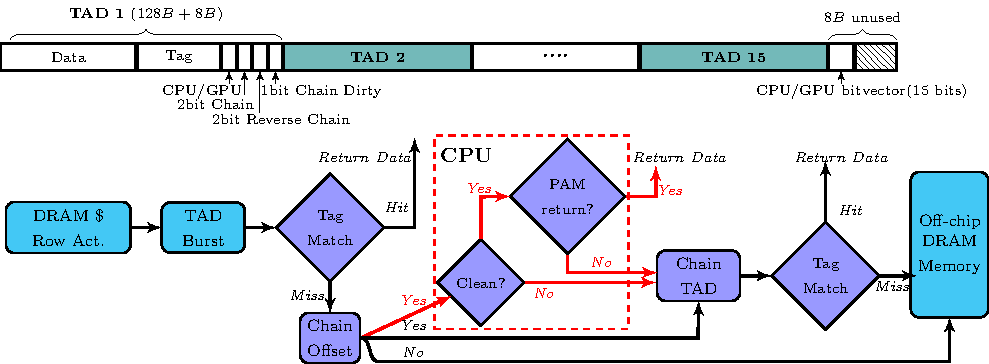
\includegraphics[scale=2.2]{chaining}
    	\caption{HAShCache Row Organization and Access Path of a request}
    \end{figure}
    \end{exampleblock}
    
% ----------------------------------------------------------------------------        
    % bypass
    \begin{exampleblock}{\circled{3} Temporal Selective Bypass Enabler : \textit{ByE}}
    	\begin{columns} [T]
    		\begin{column}{0.6\linewidth}
    	    \begin{itemize}
    	    	\item \emph{OBJECTIVE:} Utilize the idle DRAM bandwidth
    	    	\item Bypass CPU requests to clean cache lines and cache misses
    	    	\item \emph{Achieved} using a \textit{Counting Bloom Filter} that tracks dirty lines in cache
    	    	\item Overhead: 256KB (0.4\% of cache capacity)
			    \item Adjoining Fig shows working of HAShCache + ByE
    	    \end{itemize}     			
    		\end{column}
    		\begin{column}{0.4\linewidth}
    			\begin{figure}
					\centering
    			    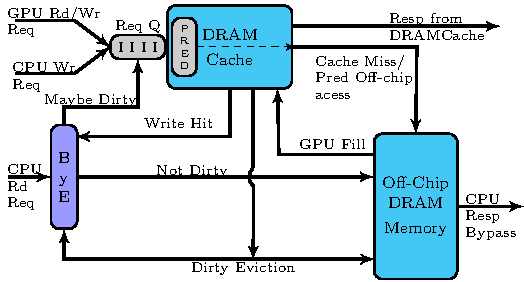
\includegraphics[scale=1.9]{bloom}
    			\end{figure}
    	    \end{column}
    	\end{columns}
	\end{exampleblock}       
% ----------------------------------------------------------------------------    
\begin{exampleblock}{Conclusion}
\vspace{-0.1em}
\begin{itemize}
\item HAShCache is heterogeneity aware and improves system throughput and achieves better resource utilization
\item Spatial Occupancy Control improves performance of CPU by 44\% by trading off just 6\% of GPU performance
\item Temporal Bypass improves performance of CPU by 48\% while sacrificing just 3\% of GPU performance 
\item Overall, addition of a stacked DRAM\$ improves CPU and GPU performance by 211\% and 20\% over a IHS baseline system with no stacked DRAM
\end{itemize}

\end{exampleblock}
\end{column}

\end{columns}
\iffalse
\begin{columns}[t]
\begin{column}{.97\linewidth}
\begin{exampleblock}{Results \& Conclusion}
	\begin{columns}[t]
		\begin{column}{.32\linewidth}
		    \begin{figure}
		    	\includegraphics[scale=3]{../graphs/results-cpu}
		    \end{figure}
		\end{column}
		\begin{column}{.32\linewidth}
		    \begin{figure}
		    	\includegraphics[scale=3]{../graphs/results-gpu}
		    \end{figure}
		\end{column}		
		\begin{column}{.32\linewidth}
			asfjasdkjf
		\end{column}				
	\end{columns}

\end{exampleblock}
\end{column}
\end{columns}
\fi
\end{frame}

\end{document}
